\documentclass[14pt,a4paper]{report}  %紙張設定
\usepackage{xeCJK}%中文字體模組
%\setCJKmainfont{標楷體} %設定中文字體
\setCJKmainfont{MoeStandardKai.ttf}
%\newfontfamily\sectionef{Times New Roman}%設定英文字體
\newfontfamily\sectionef{Nimbus Roman}
\usepackage{enumerate}
\usepackage{amsmath,amssymb}%數學公式、符號
\usepackage{amsfonts} %數學簍空的英文字
\usepackage{graphicx, subfigure}%圖形
\usepackage{fontawesome5} %引用icon
\usepackage{type1cm} %調整字體絕對大小
\usepackage{textpos} %設定文字絕對位置
\usepackage[top=2.5truecm,bottom=2.5truecm,
left=3truecm,right=2.5truecm]{geometry}
\usepackage{titlesec} %目錄標題設定模組
\usepackage{titletoc} %目錄內容設定模組
\usepackage{textcomp} %表格設定模組
\usepackage{multirow} %合併行
%\usepackage{multicol} %合併欄
\usepackage{CJK} %中文模組
\usepackage{CJKnumb} %中文數字模組
\usepackage{wallpaper} %浮水印
\usepackage{listings} %引用程式碼
\usepackage{hyperref} %引用url連結
\usepackage{setspace}
\usepackage{lscape}%設定橫式
\lstset{language=Python, %設定語言
		basicstyle=\fontsize{10pt}{2pt}\selectfont, %設定程式內文字體大小
		frame=lines,	%設定程式框架為線
}
%\usepackage{subcaption}%副圖標
\graphicspath{{./../images/}} %圖片預設讀取路徑
\usepackage{indentfirst} %設定開頭縮排模組
\renewcommand{\figurename}{\Large 圖.} %更改圖片標題名稱
\renewcommand{\tablename}{\Large 表.}
\renewcommand{\lstlistingname}{\Large 程式.} %設定程式標示名稱
\hoffset=-5mm %調整左右邊界
\voffset=-8mm %調整上下邊界
\setlength{\parindent}{3em}%設定首行行距縮排
\usepackage{appendix} %附錄
\usepackage{diagbox}%引用表格
\usepackage{multirow}%表格置中
%\usepackage{number line}
%=------------------更改標題內容----------------------=%
\titleformat{\chapter}[hang]{\center\sectionef\fontsize{20pt}{1pt}\bfseries}{\LARGE 第\CJKnumber{\thechapter}章}{1em}{}[]
\titleformat{\section}[hang]{\sectionef\fontsize{18pt}{2.5pt}\bfseries}{{\thesection}}{0.5em}{}[]
\titleformat{\subsection}[hang]{\sectionef\fontsize{18pt}{2.5pt}\bfseries}{{\thesubsection}}{1em}{}[]
%=------------------更改目錄內容-----------------------=%
\titlecontents{chapter}[11mm]{}{\sectionef\fontsize{18pt}{2.5pt}\bfseries\makebox[3.5em][l]
{第\CJKnumber{\thecontentslabel}章}}{}{\titlerule*[0.7pc]{.}\contentspage}
\titlecontents{section}[18mm]{}{\sectionef\LARGE\makebox[1.5em][l]
{\thecontentslabel}}{}{\titlerule*[0.7pc]{.}\contentspage}
\titlecontents{subsection}[4em]{}{\sectionef\Large\makebox[2.5em][l]{{\thecontentslabel}}}{}{\titlerule*[0.7pc]{.}\contentspage}
%=----------------------章節間距----------------------=%
\titlespacing*{\chapter} {0pt}{0pt}{18pt}
\titlespacing*{\section} {0pt}{12pt}{6pt}
\titlespacing*{\subsection} {0pt}{6pt}{6pt}
%=----------------------標題-------------------------=%             
\begin{document} %文件
\sectionef %設定英文字體啟用
\vspace{12em}
\begin{titlepage}%開頭
\begin{center}   %標題  
\makebox[1.5\width][s]
{\fontsize{24pt}{2.5pt}國立虎尾科技大學}\\[18pt]
\makebox[1.5\width][s]
{\fontsize{24pt}{2.5pt}工程學院機械設計工程系}\\[18pt]
\makebox[1.5\width][s]
{\fontsize{24pt}{2.5pt}專題製作報告}\\[18pt]
%設定文字盒子 [方框寬度的1.5倍寬][對其方式為文字平均分分布於方框中]\\距離下方18pt
\vspace{6em} %下移
\fontsize{30pt}{1pt}\selectfont\textbf{有限元素法在四足機器人設計上的應用}\\
\vspace{1em}
\sectionef\fontsize{30pt}{1em}\selectfont\textbf
{
\vspace{0.5em}
Application of Finite Element Method
\vspace{0.5em}
to
 \vspace{0.5em} 
Quadruped Robot Design}
 \vspace{2em}
%=---------------------參與人員-----------------------=%             
\end{center}
\begin{flushleft}
\begin{LARGE}

\hspace{32mm}\makebox[5cm][s]
{指導教授:\quad 嚴\quad 家\quad 銘\quad 老\quad 師}\\[6pt]
\hspace{32mm}\makebox[5cm][s]
{班\qquad 級:\quad 四\quad 設\quad 三\quad 乙}\\[6pt]
\hspace{32mm}\makebox[5cm][s]
{學\qquad 生:\quad 楊\quad 子\quad 頡\quad(40923231)}
\\[6pt]
\hspace{32mm}\makebox[5cm][s]
{\hspace{36.5mm}楊\quad 建\quad 霖\quad(40923233)}\\[6pt]
\hspace{32mm}\makebox[5cm][s]
{\hspace{36.5mm}詹\quad 侑\quad 儒\quad(40923235)}\\[6pt]
\hspace{32mm}\makebox[5cm][s]
{\hspace{36.5mm}蔡\quad 宗\quad 瑋\quad(40923240)}\\[6pt]
%設定文字盒子[寬度為5cm][對其方式為文字平均分分布於方框中]空白距離{36.5mm}\空白1em
\end{LARGE}
\end{flushleft}
\vspace{6em}
\fontsize{18pt}{2pt}\selectfont\centerline{\makebox[\width][s]
{中華民國\hspace{3em} 
112 \quad 年\quad 6\quad 月}}
\end{titlepage}
\newpage
%=---------------專題製作合可證明---------------------=%
 {\renewcommand\baselinestretch{1.4}\selectfont %設定以下行距
 {\begin{center}
    {\fontsize{20pt}{2.5pt} {國立虎尾科技大學 \qquad 機械設計工程系}\\[8pt]{學生專題製作合格認可證明}\\
    \hspace*{\fill} \\ %似enter鍵換行
    \par}
     \end{center}}
    {\begin{textblock}{60}(1.85,0.8)
    \noindent \fontsize{15pt}{16pt}\selectfont 專題製作修習學生\enspace:\quad
    {\begin{minipage}[t]{10em}\underline{四設三乙\enspace 40923231\enspace 楊子頡}\\ \underline{四設三乙\enspace 40923233\enspace 楊建霖}\\ \underline{四設三乙\enspace 40923235\enspace 詹侑儒}\\ \underline{四設三乙\enspace 40923240\enspace 蔡宗瑋}\\ %下劃線符號指令
    \end{minipage}}
         \par} %結束指定行距
    {\renewcommand\baselinestretch{1.2}\selectfont %設定以下行距
    {\begin{textblock}{30}(1.8,4)
    \noindent \fontsize{16pt}{16pt}\selectfont 專題製作題目\enspace :有限元素法在四足機器人設計上的應用
    \hspace*{\fill} \\
    \hspace*{\fill} \\
    \noindent \fontsize{16pt}{16pt}\selectfont 經評量合格,特此證明
    \hspace*{\fill} \\
    \hspace*{\fill} \\
    \noindent \fontsize{16pt}{16pt} \makebox[6em][s]{評審委員}\enspace:\quad
    {\begin{minipage}[t]{6em} \underline{            }\\[16pt] \underline{            }\\[16pt] \underline{            }\\
    \end{minipage}}
    \end{textblock}}
    {\begin{textblock}{10}(1.8,9)
    {\begin{flushleft}
    \fontsize{16pt}{16pt}\selectfont \makebox[6em][s]{指導老師}\enspace:\quad \underline{            }\\[10pt]
    \fontsize{16pt}{16pt}\selectfont \makebox[6em][s]{系主任}\enspace:\quad \underline{            }\\
    \hspace*{\fill} \\
    \fontsize{16pt}{2.5pt}\selectfont \makebox[12em][s]{中華民國一一貳年}\hspace{2pt}
    \fontsize{16pt}{2.5pt}\selectfont\makebox[8em][s]{六月二十日}
    \end{flushleft}}
    \end{textblock}}
    \end{textblock}}
     \par} %結束指定行距
     \newpage

%=------------------------摘要-----------------------=%
\renewcommand{\baselinestretch}{1.5} %設定行距
\pagenumbering{roman} %設定頁數為羅馬數字
\clearpage  %設定頁數開始編譯
\sectionef
\addcontentsline{toc}{chapter}{摘~~~要} %將摘要加入目錄
\begin{center}
\LARGE\textbf{摘~~~要}\\
\end{center}
\begin{flushleft}
\fontsize{14pt}{20pt}\sectionef\hspace{12pt}\quad 本專題主要研究有限元素法(FEM),由於近代計算機快速的發展,數值計算、開發環境、生程式設計等,都有公司或個人創作者製作軟體進行分析、計算,藉由這些軟體我們將對四足機器人進行生成式設計並且觀察其受力情況。\\[14pt]
\fontsize{14pt}{20pt}\sectionef\hspace{12pt}\quad 以四足機器人為例,將結構以剛體狀況導入CoppeliaSim進行動作模擬後,求出最大反力分別帶入Ansys和Solid Edge,並在此轉換為柔性結構,進行有限元素(FEM)分析,評估各柔性結構下分析的應力、應變等受力情況,對其做生成式設計以簡化模組,在保有強度的同時減輕重量造成最少的能源浪費。並嘗試透過網路展示CoppeliaSim機器人運動情況,證明其設計可行性。\\[12pt]

\end{flushleft}
\begin{center}
\fontsize{14pt}{20pt}\selectfont 關鍵字:偏微分方程(PDE)、有限元素分析(PEM)、CoppeliaSim、Ansys、Solid Edge
\end{center}
\newpage

%=--------------------Abstract----------------------=%
\renewcommand{\baselinestretch}{1.5} %設定行距
\addcontentsline{toc}{chapter}{Abstract} %將摘要加入目錄
\begin{center}
\LARGE\textbf\sectionef{Abstract}\\
\begin{flushleft}
\fontsize{14pt}{16pt}\sectionef\hspace{12pt}\quad The main focus of this project is on the Finite Element Method (FEM). With the rapid development of modern computers, numerical calculations, development environments, and software programming, various companies or individual creators have developed software for analysis and calculations. With the help of these software programs, we will perform generative design on a quadruped robot and observe its structural integrity under various load conditions.\\[12pt]

\fontsize{14pt}{16pt}\sectionef\hspace{12pt}\quad Taking the quadruped robot as an example, we will import the structure as a rigid body into CoppeliaSim for motion simulation. After obtaining the maximum reaction forces, we will input them into Ansys and Solid Edge for further analysis. The rigid structure will then be converted into a flexible structure to perform Finite Element Method (FEM) analysis. We will evaluate the stress, strain, and other load conditions for each flexible structure to assess their performance. Through generative design, we aim to simplify the modules while maintaining their strength and minimizing energy waste caused by excessive weight. Additionally, we will attempt to showcase the motion of the robot in CoppeliaSim through online demonstrations to prove the feasibility of the design.\\
\end{flushleft}
\begin{center}
\fontsize{14pt}{16pt}\selectfont\sectionef Keywords: partial differential equation (PDE), finite element analysis (PEM), CoppeliaSim, Ansys, Solid Edge.
\end{center}

\newpage
%=------------------------誌謝----------------------=%
\addcontentsline{toc}{chapter}{誌~~~謝}
\centerline\LARGE\textbf{誌~~謝}\\
\begin{flushleft}
\fontsize{14pt}{2.5pt}\hspace{12pt}\quad 本專題能完成有著許多人員的幫忙,大四學長他們不吝嗇地將往年的製作經驗傳授給我們,讓我們在製作的時候少走了許多錯路,還總是貼心找出重點提醒我們可以加以描述。再來是我們的指導教授嚴家銘教授,他提供了多方面的資訊,拋出問題並給予建議,擬定了我們小組有限元素法研究和學習方向,開會也時常提出建議以及未來發展,得以順利解決遇到的技術問題,同時也給了相當程度的自由,讓小組得以有彈性去尋探索及摸索,而本專題組員也充分地付出了許多,讓專題研究能順利完成,從中獲益良多,特此感謝。
\end{flushleft}
\newpage
%=------------------------目錄----------------------=%
\renewcommand{\contentsname}{\centerline{\fontsize{18pt}{\baselineskip}\selectfont\textbf{目\quad 錄}}}
\tableofcontents  %目錄產生
\newpage
%=------------------圖表目錄產生----------------------=%
\renewcommand{\listfigurename}{\centerline{\fontsize{18pt}{\baselineskip}\selectfont\textbf{圖\quad 目\quad 錄 }}}
\newcommand{\loflabel}{圖} %定義\loflabel 文字為圖
\renewcommand{\numberline}[1]{\loflabel~#1\hspace*{0.5em}}
\listoffigures
%\newcommand{\captioname}{圖}
\newpage
\renewcommand{\listtablename}{\centerline{\fontsize{18pt}{\baselineskip}\selectfont\textbf{表\quad 目\quad 錄 }}}
\newcommand{\lotlabel}{表} %定義\lotlabel 文字為表
\renewcommand{\numberline}[1]{\lotlabel~#1\hspace*{0.5em}}
\listoftables

\end{center}
%=-------------------------內容----------------------=%
\chapter{緒論}
\renewcommand{\baselinestretch}{10.0} %設定行距
\pagenumbering{arabic} %設定頁號阿拉伯數字
\setcounter{page}{1}  %設定頁數
\fontsize{14pt}{2.5pt}\sectionef

\section{研究動機與背景}
材料分析軟體的應用在機械領域愈來越廣泛,能夠將繪製零件進行分析,但卻鮮少人知道材料分析是怎麼進行的,背後所引用的代碼、原理的東西。本專題研究方向將由四足機器人作為設計主題,提供所需參數,將有限元素分析的公式套入並計算,對建模進行力學分析,用於設計優化,將透過本專題了解。(圖.\ref{fig.pong_gym})。\\
------------------------------------------------------
\begin{figure}[hbt!]
\begin{center}
\includegraphics[angle=90,width=10cm]{冰球機}
\caption{\Large 實體的冰球機}\label{fig.冰球機}
\end{center}
\end{figure}
-------------------------------------------------------
\begin{figure}[hbt!]
\begin{center}
\includegraphics[angle=90,width=10cm]{origin}
\caption{\Large 虛擬環境簡化後的冰球機}\label{fig.模擬冰球機}
\end{center}
\end{figure}
---------------------------------------------------------
\begin{figure}[hbt!]
\begin{center}
\includegraphics[height=8cm]{pong_gym}
\caption{\Large Gym的Pong game}\label{fig.pong_gym}
\end{center}
\end{figure}
--------------------------------------------------------------

\section{研究目的與方法}
本專題研究是以有限元素法有限元分析,Solid Edge繪出3D模型,並加入材質及各式力,測試不同部位所得出的物體模型的模擬分析,求出各個物理問題(應力、應變、變形等)。\\

以四足機械狗為模型,由solid edge建立3D模型,導入CoppeliaSim模擬環境,透過軟體的模擬功能,測試模型可行性,找出機器狗在運動時各部位的軌跡並找出反力為何。\\

接著利用Solid Edge分析,利用軟體中的有限元素法及各式方程式結合成的線性方程、進行代數求解、模擬,觀察、分析此模型在受力後的反應,篩選出適合的材料及形狀,透過此部分驗證材料的性質是否能夠負荷並擁有某些脆弱點,透過以上步驟可驗證實際運用上的此設計是否可行也可以讓設計者盡早發現錯誤並修正。\\
 -------------------------------------------------------------
\begin{figure}[hbt!]
\begin{center}
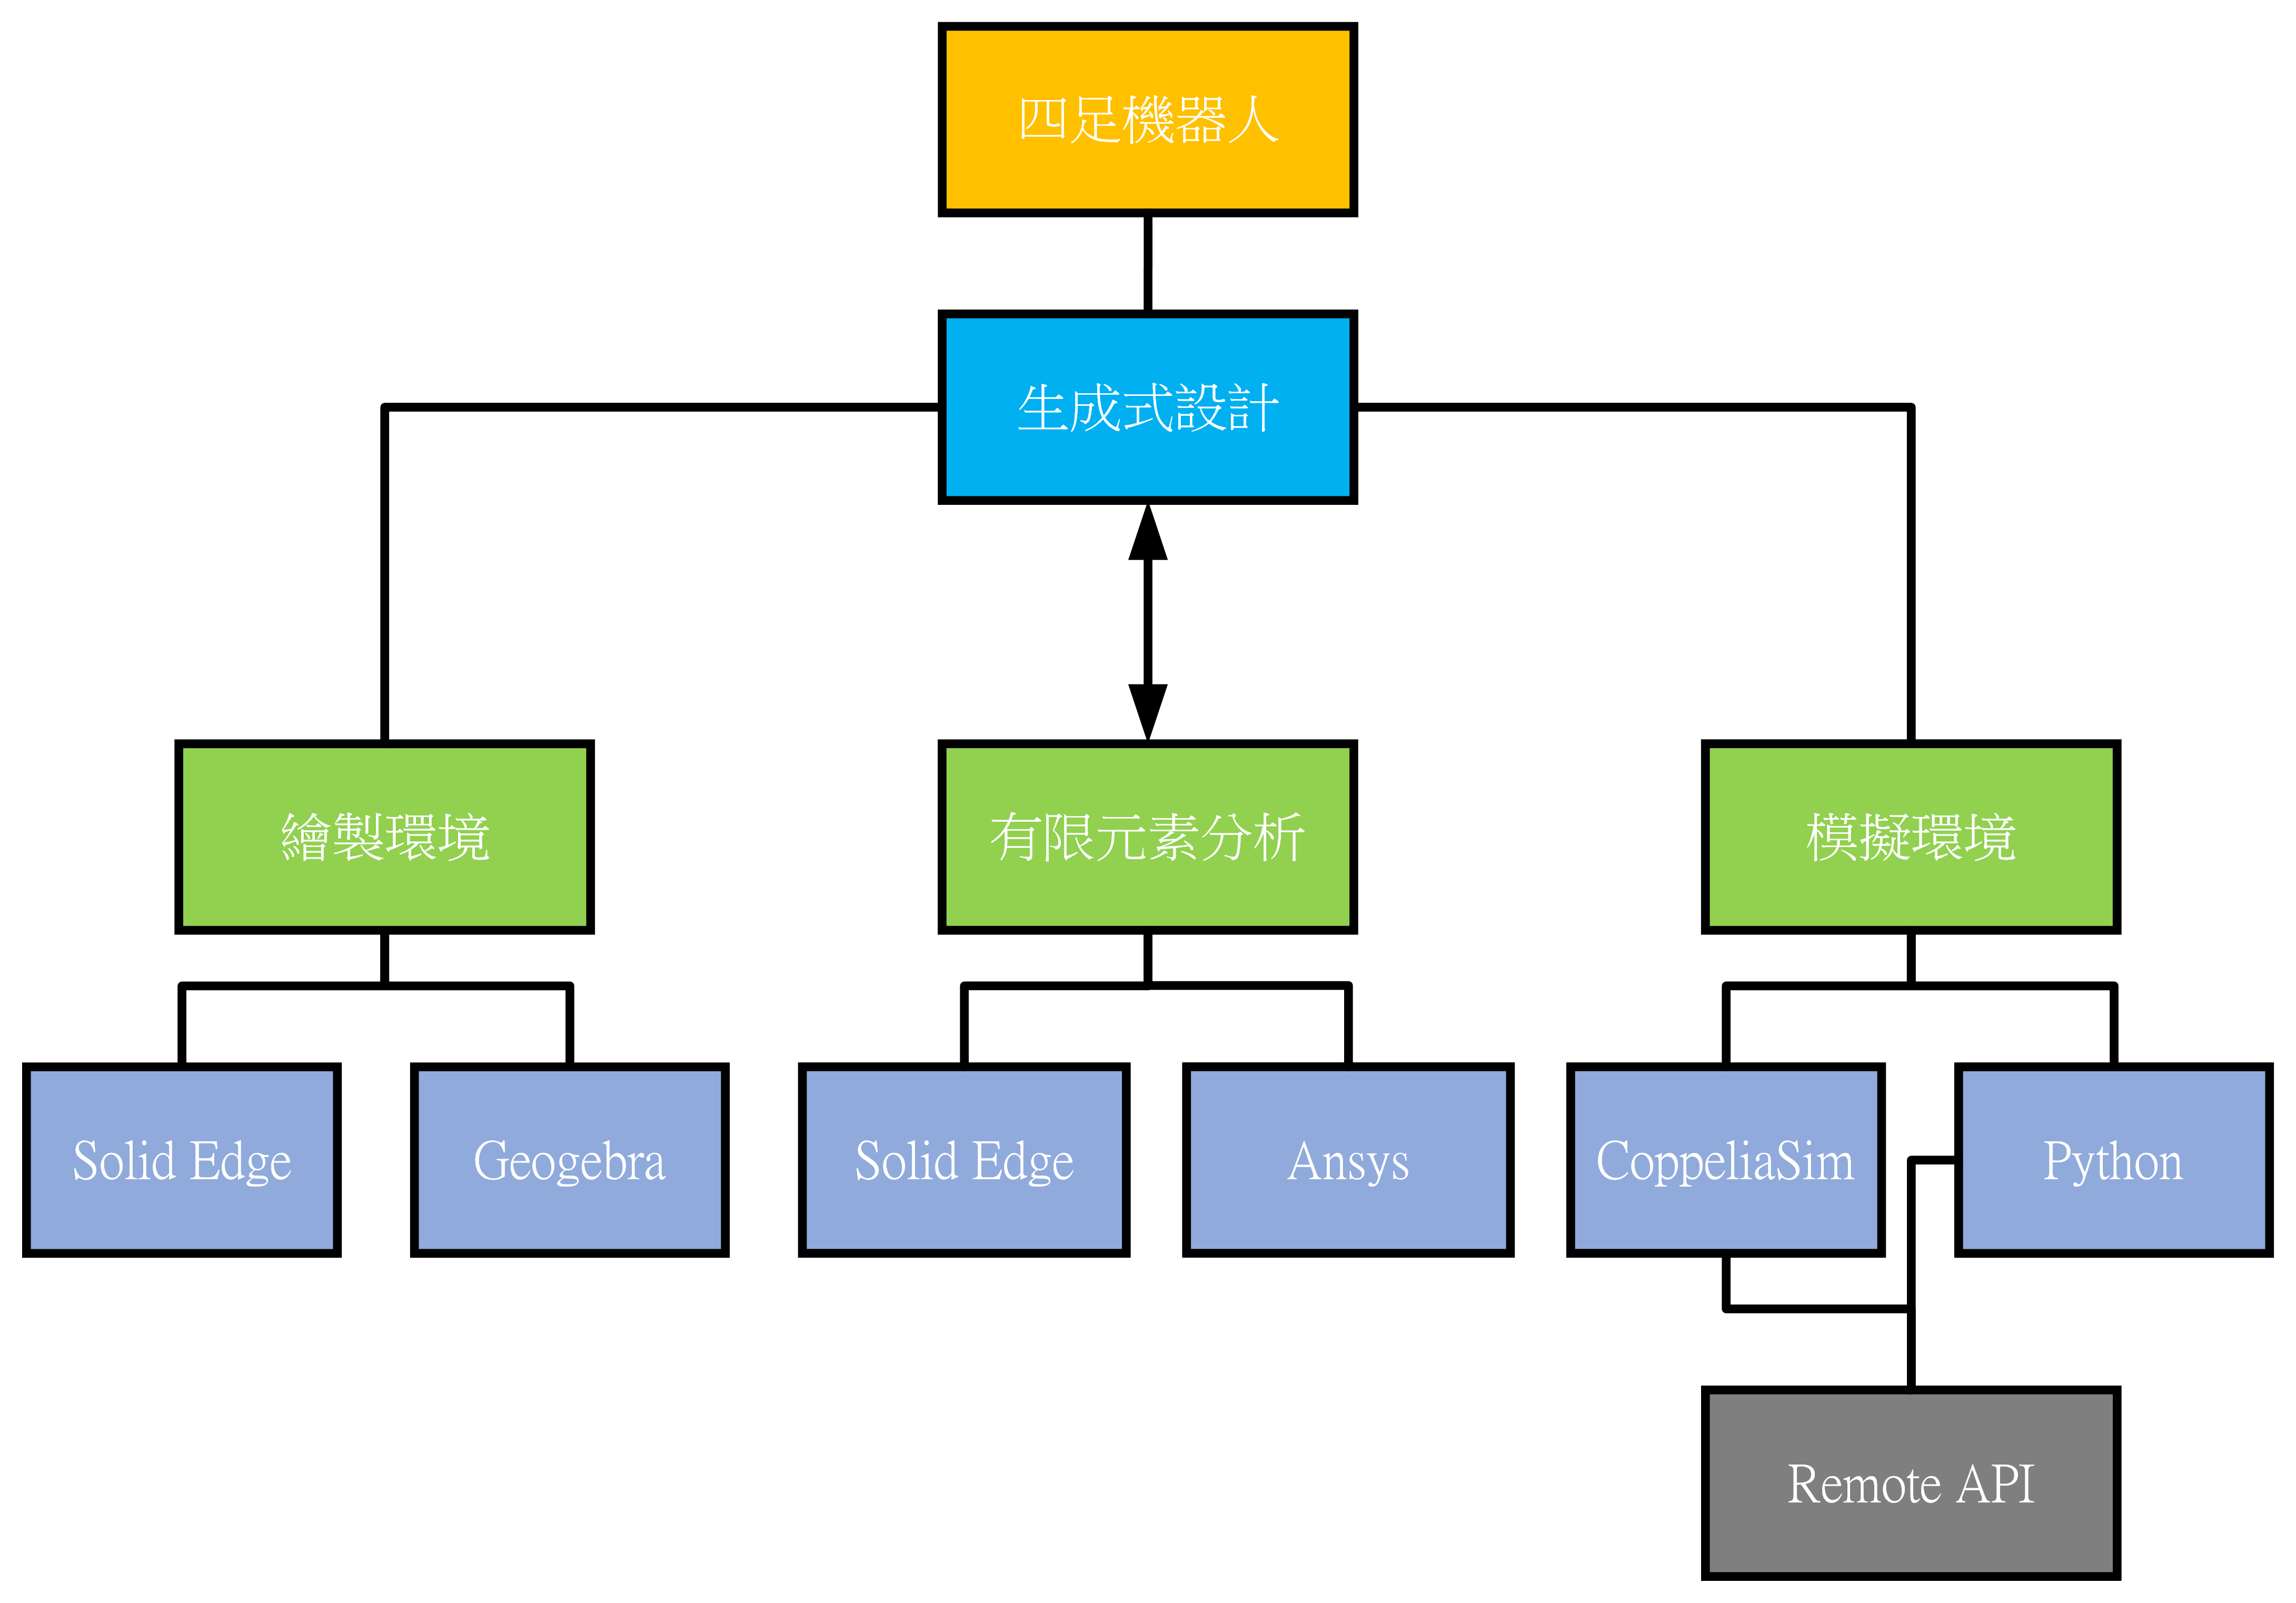
\includegraphics[width=15cm]{研究架構}
\caption{\Large 研究架構 }
\label{研究架構 }
\end{center}
\end{figure}
-------------------------------------------------------

\section{未來展望}

透過此研究可以求解出模型所受外力影響的數值變化,若之後可以對軟體輸入參數及設計因子,則軟體可以在所設定的範圍中透過計算產生設計者所需的模型並且,不再只局限於設計者的想像力,或是透過手機的日漸進步的激光雷達掃描系統,可以讓許多用戶都可以輕易地使用分析功能。\\

\section{分析說明}

模型進行運動分析後,透過求出的反力做為設計參數,帶入到至應力分析軟體中,並帶入合適的材料,通過預設的安全係數為最終目標。\\

\renewcommand{\baselinestretch}{0.5} %設定行距

\chapter{有限元素法}
用於求解偏微分方程或積分方程組數值求解,將大型物理系統細分為更小、更簡單的部分,稱為有限元,通過在空間維度上進行特定的空間離散化簡化連續變量的複雜性,有限元素法通過最小化關聯的誤差函數,使用來自變異演算的變異方法來近似求,來實現用於複雜的工程結構或物理系統的行為和性能。\\

%---------------------第二章/基本概念及假設假定-------------------------%
\section{基本概念及假設假定}

1.有限元素:通常由三角形或者四邊形等形成結構的區域。\\

2.節點:每個元素的角落或中心點,用於連接元素之間的邊界條件和解決方程。\\

3.自由度: 節點上變量的個數,例如位移的節點自由度為3,表示單個節點擁有三個坐標方向的位移,又例如熱分析時節點自由度為1,表示某個節點處的溫度。\\

4.網格:由數個元素經由節點連接所組成,用以表示在需求解的區域上。\\

5.變形:系統在外力的影響下發生的形變,經過分析後計算每個元素的變形及變形之間的相互引響預測整得系統的變形及應力、各種參數的分布。\\

6.離散化:將物理系統或結構等連續變量通過計算轉換為數格元素的過程,目的在於減化數據,減少連續變量的複雜性,便於處理及分析。關於公式及步驟會因為模型或問題的類型不同而有不一樣的計算方式。\\

7.邊界條件:物理系統邊界上的約束和力,模擬實際問題中的條件及約束。\\

8.材料特性:物理系統(模型)的材料性質,不同的材料其中的參數各為不同(彈性模數、潽淞比、極限強度、屈服強度等)。\\

\begin{figure}[hbt!]
\begin{center}
\includegraphics[width=16cm]{類神經網路架構}
\caption{\Large 類神經網路架構}\label{類神經網路架構}
\end{center}
\end{figure}
\newpage

\begin{figure}
\begin{center}
\includegraphics[width=16cm]{類神經網路架構}
\caption{\Large 類神經網路架構}
\label{類神經網路架構}
\end{center}
\end{figure}
\begin{itemize}
%=----------Sigmoid      Function----------=%
\item Sigmoid Function(圖.\ref{SigmoidFunction}):\\
$$\sigma(x)=\frac{1}{1+e^{-x}}$$

%=----------SigmoidPrime Function----------=%
$$\sigma^{'}(x)=\sigma(x)[1-\sigma(x)]$$
\begin{figure}[hbt!]
\begin{center}
\includegraphics[width=16cm]{SigmoidFunction}
\caption{\Large SigmoidFunction}\label{SigmoidFunction}
\end{center}
\end{figure}
\\
%=----------Softmax Function----------=%
\item Softmax:\\
$$S(x)=\frac{e^{x_i}}{\sum^k_{j=1}e^{x_i}}$$
%=----------Relu Function----------=%
\item ReLU Function:\\
\end{itemize}
$$f(x)=max(0,x)$$
$$if , x<0 , f(x)=0$$
$$else f(x)=x$$

%=----------Faces of Reinforcement Learning---------------=%

強化學習涵蓋範圍(圖.\ref{各領域與機器學習應用範圍}):\\
 
%======需文字補充========%
\begin{figure}[hbt!]
\begin{center}
\includegraphics[width=11cm]{Faces_of_Reinforcement_Learning}
\caption{\Large 各領域與機器學習應用範圍}
\label{各領域與機器學習應用範圍}
\end{center}
\end{figure}
%=--------The Flow of Reinforcement Learning------------=%.
\newpage
\begin{figure}[hbt!]
\begin{center}
\includegraphics[width=12cm]{The_Flow_of_Reinforcement_Learning}
\caption{\Large 強化學習架構}
\label{RL structur}
\end{center}
\end{figure}
\newpage
\begin{figure}[hbt!]
\begin{center}
\includegraphics[width=15cm]{The_entire_interaction_process}
\caption{\Large 整個互動過程}
\label{整個互動過程}
\end{center}
\end{figure}

 
%------------------圖片可共用----------------------%
\iffalse
\begin{figure}[hbt!]
\begin{center}
\includegraphics[scale=0.74]{ Reinforcement_Learning_interactions}
\caption{\Large Reinforcement Learning interactions}
\end{center}
\end{figure}
\fi
%=----Interactions with Reinforcement Learning------------=%


\begin{figure}[hbt!]
\begin{center}
\includegraphics[width=15cm]{agent}
\caption{\Large agent}
\label{agent}
\end{center}
\end{figure}
%=----Agents------------=%
\begin{flushleft}
\end{flushleft}

%--------------------------第二章/網格劃分基本原則--------------------------%
\section{網格劃分基本原則}
1. 網格數量:將決定計算經度及規模大小,一般狀況中,網格數量增加計算精度也會跟著提升,但伴隨而來的是更大的計算量,所以在制定網格大小時應權衡兩個因素。\\

2. 網格疏密:在某些變化梯度較大的部位(應力集中處),需要大密集的網格,密集往個將更好反映數據變化,反之變化梯度較小的部位則用較稀疏的網格,而不同單元之間的連接則採用特殊的過度單元或多點約束等方法連接,才能更好的分配資源,兼顧計算量何計算精度。\\

3. 網格質量:指網格型狀的合理性,質量的好壞將直接影響計算精度,質量較差的除了造成局部的計算精度偏差甚至會直接終止計算,因此在重要部位時應該確保其擁有高品質的表現。\
如果網格都是由等邊三角形、正方形、正四面體、立方六面體等組成,則求解精度可以非常接近實際值,但這種只存在於理想狀態下,實際運用卻很難做到。\\

元素質量評價有幾個指標\\

1. 單元的邊長比、面積比及體積比,理想的邊長比為1,以正三角形、正四面體、正六面體為參考基準\\

2. 扭曲度:單元內部扭轉及面外的翹曲程度\\

3. 疏密過渡:應力梯度方向和橫向過渡情況,應力集中部分應較為密集,則反之\\

4. 節點、元素排部:合理的節點及元素有助於帶入方程式計算,可以提高求解效率,並且須注意消除重複的節點及元素\\


%--------------------------第二章/有限元計算公式--------------------------%
\section{有限元計算公式}
對於有限元素法代入模型的各種問題求解,以下有著幾種計算公式。\\
%
%---------------------{有限元素應力計算公式}---------------------%
\subsection{有限元素應力計算公式}
1. 對於三角形元素而言,其計算方法如下\\
\[
\begin{aligned}
\sigma x=\left( \dfrac{1}{\Delta }\right) \times \left[ \sigma _{1}\times \left( y_{2}-y_{3}\right) +\sigma _{2}\times \left( y_{3}-y_{1}\right) +\sigma _{3}\times \left( y_{1}-y_{2}\right) \right]\\
\sigma y=\left( \dfrac{1}{\Delta }\right) \times \left[ \sigma _{1}\times \left( x_{3}-x_{2}\right) +\sigma _{2}\times \left( x_{1}-x_{3}\right) +\sigma _{3}\times \left( x_{2}-x_{1}\right) \right]\\
\tau xy=\left( \dfrac{1}{\Delta }\right) \times \left[ \tau _{1}\times \left( x_{3}-x_{2}\right) +\tau _{2}\times \left( x_{1}-x_{3}\right) +\tau _{3}\times \left( x_{2}-x_{1}\right) \right]\\
\end{aligned}
\]
其中,σx, σy, τxy 分別表示在 x, y 方向上的正應力和剪應力,σ1, σ2, σ3 表示每個節點上的應力,τ1, τ2, τ3 表示每個節點上的剪應力,Δ 表示三角形單元的面積。\\

2. 對於四邊形元素而言,其計算方法如下\\
\[
\begin{aligned}
\sigma _{x}=\left( \dfrac{1}{4t}\right) \times \left[ \sigma _{1}\times \left( y_{4}-y_{2}\right) +\sigma _{2}\times \left( y_{1}-y_{3}\right) +\sigma _{3}\times \left( y_{2}-y_{4}\right) +\sigma _{4}\times \left( y_{3}-y_{1}\right) \right]\\
\sigma _{y}=\left( \dfrac{1}{4t}\right) \times \left[ \sigma _{1}\times \left( x_{2}-x_{4}\right) +\sigma _{2}\times \left( x_{3}-x_{1}\right) +\sigma _{3}\times \left( x_{4}-x_{2}\right) +\sigma _{4}\times \left( x_{1}-x_{4}\right) \right]\\
\tau xy=\left( \dfrac{1}{4t}\right) \times \left[ \tau _{1}\times \left( x_{2}-x_{4}\right) +\tau _{2}\times \left( x_{3}-x_{1}\right) +\tau 3\times \left( x_{4}-x_{2}\right) +\tau 4\times \left( x_{1}-x_{3}\right) \right]\\
\end{aligned}
\]
其中,σx, σy, τxy 分別表示在 x, y 方向上的正應力和剪應力,σ1, σ2, σ3, σ4 表示每個節點上的應力,τ1, τ2, τ3, τ4 表示每個節點上的剪應力,t 表示四邊形單元的厚度。\\

%-------------------{有限元素應力計算公式}------------------------%
\subsection{有限元素應力計算公式}
1. 對於三角形元素而言,其計算方法如下\\
\[
\begin{aligned}
\varepsilon x=\left( \dfrac{1}{\Delta }\right) \times \left[ \varepsilon 1\times \left( y_{2}-y_{3}\right) +\varepsilon 2\times \left( y_{3}-y_{1}\right) +\varepsilon 3\times \left( y_{1}-y_{2}\right) \right]\\
\varepsilon y=\left( \dfrac{1}{\Delta }\right) \times \left[ \varepsilon 1\times \left( x_{3}-x_{2}\right) +\varepsilon 2\times \left( x_{1}-x_{3}\right) +\varepsilon 3\times \left( x_{2}-x_{1}\right) \right]\\
\gamma xy=\left( \dfrac{1}{\Delta }\right) \times \left[ \gamma _{1}\times \left( x_{3}-x_{2}\right) +\gamma _{2}\times \left( x_{1}-x_{3}\right) +r_{3}\times \left( x_{2}-x_{1}\right) \right]\\
\end{aligned}
\]
其中,εx, εy 分別表示在 x, y 方向上的應變,γxy 表示剪應變,ε1, ε2, ε3 分別表示每個節點上的應變,γ1, γ2, γ3 表示每個節點上的剪應變,Δ 表示三角形單元的面積。\\

2. 對於四邊形元素而言,其計算方法如下\\
\[
\begin{aligned}
\varepsilon _{x}=\left( \dfrac{1}{4t}\right) \times \left[ \varepsilon _{1}\times \left( y_{4}-y_{2}\right) +\varepsilon _{2}\times \left( y_{1}-y_{3}\right) +\varepsilon _{3}\times \left( y_{2}-y_{4}\right) +\varepsilon _{4}\times \left( y_{3}-y_{1}\right) \right]\\
\varepsilon _{y}=\left( \dfrac{1}{4t}\right) \times \left[ \varepsilon _{1}\times \left( x_{2}-x_{4}\right) +\varepsilon _{2}\times \left( x_{3}-x_{1}\right) +\varepsilon _{3}\times \left( x_{4}-x_{2}\right) +\varepsilon _{4}\times \left( x_{1}-x_{4}\right) \right]\\
\gamma xy=\left( \dfrac{1}{4t}\right) \times \left[ \gamma _{1}\times \left( x_{2}-x_{4}\right) +\gamma _{2}\times \left( x_{3}-x_{1}\right) +\gamma 3\times \left( x_{4}-x_{2}\right) +\gamma 4\times \left( x_{1}-x_{3}\right) \right]\\
\end{aligned}
\]
其中,εx, εy 分別表示在 x, y 方向上的應變,γxy 表示剪應變,ε1, ε2, ε3, ε4 分別表示每個節點上的應變,γ1, γ2, γ3, γ4 表示每個節點上的剪應變,t 表示四邊形單元的厚度。\\

%-----------有限元素動力學分析公式-------------%
\subsection{有限元素動力學分析公式}
1. 結構的運動方程\
在有限元素動力學分析中,結構的運動方程通常採用以下形式表示:\\
\[
\begin{aligned}
\left[ M\right] \times \left\{ u''\right\} +\left[ C\right] \times \left\{ u'\right\} +\left[ K\right] \times \left\{ u\right\} =\left\{ F\left( t\right) \right\}\\
\end{aligned}
\]
其中,[M]、[C] 和 [K] 分別表示結構的質量、阻尼和剛度矩陣,{¨u}、{˙u} 和 {u} 分別表示結構的加速度、速度和位移矢量,{F(t)} 表示結構受到的外部激勵矢量。\\

2. 求解運動方程\
通過對運動方程進行離散化處理,可以得到結構的位移、速度和加速度的數值解。通常採用時間步進法求解運動方程,其中最常用的是 Newmark-β 方法,其求解公式如下:\\
\[
\begin{aligned}
\left\{ u\left( t+\Delta t\right) \right\} =\left\{ u\left( t\right) \right\} +\left\{ u'\left( t\right) \right\} \Delta t+\left( \dfrac{1}{2}-\beta \right) \times \left\{ u''\left( t\right) \right\} \Delta t^{2}+\beta \left\{ u''\left( t+\Delta t\right) \right\} \Delta t^{2}\\
\left\{ u'\left( t+\Delta t\right) \right\} =\left\{ u'\left( t\right) \right\} +\left( 1-\gamma \right) \times \left\{ u''\left( t\right) \right\} \Delta t+\gamma \left\{ u''\left( t+\Delta t\right) \right\} \Delta t\\
\end{aligned}
\]
其中,β 和 γ 是時間步進法的參數,其取值需要根據求解的精度和計算效率進行權衡。\\

3. 應力計算公式\
在求解結構動態響應的過程中,通常需要計算結構內部的應力分佈情況。對於有限元素動力學分析而言,常用的應力計算公式是根據結構位移和應變之間的關係推導而來的。具體來說,可以採用以下公式進行應力計算:\\
\[
\begin{aligned}
\left\{ \sigma \right\} =\left[ D\right] \times \left\{ \varepsilon \right\}
\end{aligned}
\]
其中,{σ} 和 {ε} 分別表示應力和應變矢量,[D] 表示材料的彈性剛度矩陣,其數值可以根據材料的力學性質進行計算。\\

%-----------有限元素疲劳分析公式------------%
\subsection{有限元素疲勞分析公式}
1. 疲勞壽命計算公式\
在有限元素疲勞分析中,常用的疲勞壽命計算公式是基於線性累積損傷理論的公式,其表示形式如下:\\
\[
\begin{aligned}
N=\dfrac{1}{\left( \Delta ^{\sigma }/2S\right) ^{m}}\\
\end{aligned}
\]
其中,N 表示疲勞壽命,Δσ 表示應力幅值,S 表示材料的疲勞極限,m 是材料的疲勞指數,其數值可以根據材料的力學性質進行計算。\\

2. 應力計算公式\
在有限元素疲勞分析中,需要對結構的應力分佈進行計算。常用的應力計算公式是基於虛功原理推導而來的,其表示形式如下:\\
\[
\begin{aligned}
\int \left\{ \sigma \right\} T\left\{ \delta \varepsilon \right\} dV=\int \left\{ f\right\} T\left\{ \delta u\right\} dV+\int \left\{ T\right\} T\left\{ \delta u\right\} dS\\
\end{aligned}
\]
其中,{σ} 和 {ε} 分別表示應力和應變矢量,{f} 表示結構受到的外部載荷矢量,{u} 表示結構的位移矢量,{T} 表示結構的邊界條件。\\

3. 疲勞壽命修正公式\
在實際應用中,疲勞壽命計算公式需要考慮多種因素的影響,如應力比、材料強度和載荷歷史等。常用的疲勞壽命修正公式包括 Goodman、Soderberg、Walker 和 Morrow 等,其表示形式可以根據具體的應用要求進行選擇。\\

%=========表格=========%
\begin{center}
\begin{tabular}[c]{ccc}    
%\multicolumn{1}{r}{MRP}
 MRP & $\longleftrightarrow$ & MDP\\
\hline
$P^{\pi}(s's)$ & = & $\sum_{a\in A}\pi (a|s)P(s'|s, a)$\\
$P^{\pi}(s)$ & = & $\sum_{a\in A}\pi (a|s)P(s, a)$\\
\includegraphics[height=3cm]{MRP}&&\includegraphics[height=3cm]{MDP}\\
\hline
\end{tabular}
\end{center}
\hspace{15pt}
 
state value function(狀態值方程式)$v^{\pi}(s)$\\
$$v^{\pi}(s) = \mathbb{E}[G_t|s_t=s]$$
$$= \mathbb{E}[R_{t+1}+\gamma v^{\pi}(s_{t+1})|s_t=s]$$
$$= \sum_{a\in A}\pi (a|s)q^{\pi}(s, a)$$
\begin{figure}[hbt!]
\begin{center}
\includegraphics[width=8cm]{s_to _s}
\caption{$v^{\pi}$程序圖}
\label{fig.s_to_s}
\end{center}
\end{figure}
$$v^{\pi}(s) = \sum_{a\in A}\pi (a|s)(R(s, a)+\gamma \sum_{s'\in s}P(s'|s, a)v^{\pi}(s'))$$
\newpage
state value function(狀態值方程式)$q^{\pi}(s)$
$$v^{\pi}(s) = \mathbb{E}[G_t|s_t=s]$$
$$= \mathbb{E}[R_{t+1}+\gamma v^{\pi}(s_{t+1})|s_t=s]$$
$$= \sum_{a\in A}\pi (a|s)q^{\pi}(s, a)$$
\begin{figure}[hbt!]
\begin{center}
\includegraphics[width=8cm]{Q_pi function}
\caption{$q^{\pi}$程序圖}
\label{fig.q_pi}
\end{center}
\end{figure}
$$q^\pi(s, a)=R(s, a)+\gamma\sum_{s'\in S}P(s'|s, a)\sum_{a'\in A}\pi(a'|s')q^{\pi}(s', a')$$
\newpage
%-----------------------第2章/分析步驟--------------------------%
\section{分析步驟}

1.建立幾何模型:將需求解的問題繪製成幾何模型,以透過二維或三維帶入\\

2.離散化:將模型分成數個元素\\

3.導入有限元方程:對每個需求解的模型或問題不相同,根據力學性質或物理方程帶入相應的關西式(應力、應變、變形、熱傳等)\\

4.裝配方程組:將所有單元方程組裝成一個大的線性方程,對問題進行代數求解\\

5.求解方程組:透過線性方程,得到節點處的位移及負載等相關訊息\\

6.後處理:對求解結果進行誤差分析及驗證\\
\newpage

\begin{figure}[hbt!]
\begin{center}
\includegraphics[width=15cm]{policy gradient原理}
\caption{\Large Policy Gradient原理}
\label{Policy Gradient原理}
\end{center}
\end{figure}
\newpage

\chapter{四足機器人}
%--------------------應用範圍反作用--------------------%
\section{應用範圍反作用}
四足機器人為一種模仿動物四肢運動方式的機器人,利用電子元件驅動機械臂可以做出許多人類難以完成的任務,同時為人們帶來許多樂趣及益處。可大致上分為以下幾項\\

1.軍事:四足機器人有良好的機械性能,搭配著電子控制系統,可以輕鬆在各地形中運輸物品及人員,透過感測器的回饋,調適馬達的行程及出力大小,在戰場中穿梭及運輸補給品,或是在搜救行動也可以當作先鋒隊,減少搜救人員的危險性並增加搜救的效率。\\

2.工業:減少作業人員在負重或高溫及有毒物質的危害中職業傷害,並保持高效的運作,減少工業中的資源浪費,在醫療機構中可以減少醫護人員的職業爆露、並經過充分消毒後也可以成為照顧病人的工具之一。\\

3.民生:四足機器人也可以當作寵物飼養,陪伴主人進行各種活動,並且可以執行各種指令,在主人發生意外時或偉危險發生時可以主動通報主人或救護單位,也可幫助年老或行動不便者的各種需求,也可以模組化各部件,讓人們可以依照需求進行各式改裝及編成。\\

隨著電腦的普及,各式各樣的編程軟體如雨後春筍般誕生,並且計算機語言也日益簡化,讓更多使用者可以越來越輕鬆的使用,網路上也有許多工程師分享開源的程式可以參考及學習。\\[6pt]

%----------------機械手臂運動學模型---------------%
\section{機械手臂運動學模型}

在步行結構設計之初,設計者通常通過模仿生物腿部來創造不同的機械模型,不同型態的機械模型都有其各自特性,對於連接機構的運動控制,一般來說,腿部的機械結構不能過於複雜,過多的機械零件需要較精細的控制元件及設計、製造成本,對於控制運動軌跡來說較於不益,以三連桿及四連桿閉環機構介紹。\\
\subsection{步行結構運動學模型介紹}
1.三連桿閉環連接機構\\
為三個結構組成,以生物的身體構造解釋,可分為髖關節、大腿、小腿,結構以一個關節連接本體,對於此種機構,優點在於結構較為緊湊、簡單,通過控制三連桿節的旋轉角度,控制尾端的位置及姿態,達到目標位置及姿態。\\

2.四連桿閉環連接機構\\
為四個結連桿組成一個不規則四邊型 ,有著兩個馬達分別驅動A、B桿,通過A、B桿的搖擺可以讓姿態有大幅度的運動,此機構較為複雜,需要精細的控制才能實現較穩定的運動,但有著能承受較大附載的優勢,對於運動穩定性也有著良好的表現,也是這個專題研究為何會選擇此機構的原因之一。\\

%-------------四連桿機構運動學模型---------------%
\section{四連桿機構運動學模型}

四連桿機構最早可以追朔到19世紀末的機械工程領域,用於織布機的機械結構,由四個桿件及四個轉動連接點組成,形成一個不規則的四邊形閉環,可以控制機械的運動軌跡及速度,實現自動化編織過程。
在現代,四連桿閉環機構被廣泛用於機械工業、機器人技術等領域。作為機器人的關節結構有靈活、平穩、高負載、高自由度等特性,使成為此領域重要結構之一,隨著科技的發展人們也不斷對此機構進行改進和創新、優化以滿足更多的應用需求。\\
 此四連桿透過驅動A、D軸來控制另外兩從動軸,實現運動姿態,\\

……………………四連桿目標位置公式….………………..

\subsection{順向運動學}
順向運動學公式是用以計算末端點位置及姿態的數學公式,該公式由矩陣組成,主要利用幾何關係與向量代數以求解四連桿機構的運動學參數及目標位置、速度、角度。\
首先建立四連桿機構運動學模型,設定關節角度、連桿長度、連桿偏移量等參數,接著利用上述所提到的代數和幾何關係求解步行機構的目標位置等參數。\\

\begin{figure}[hbt!]
\begin{center}
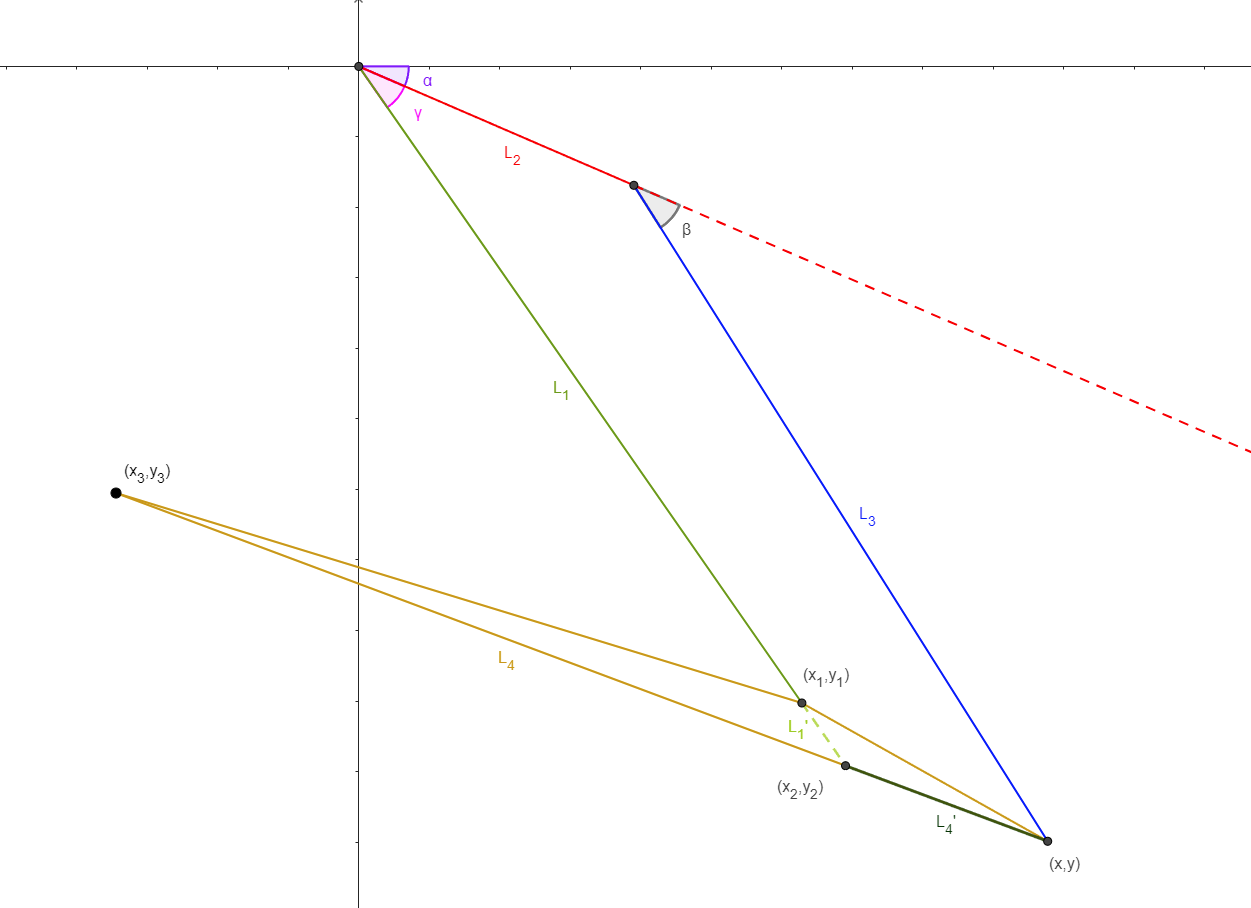
\includegraphics[width=10cm]{Forward kinematics formula}
\caption{\Large 四連趕機構}\label{Forward kinematics formula}
\end{center}
\end{figure}
    
\[
\begin{aligned}
x=L_{1}\cos \alpha +L_{2}\cos \left( \alpha +\beta \right) \\ 
y=L_{1}\sin \alpha +L_{2}\sin \left( \alpha +\beta \right) 
\end{aligned}
\]
---------------------------順向運動學公式-------------------------------


將步行機構的參數套入此公式,給定各連桿及方向和位置,接著將各關節的象隊座標矩陣相乘,即可以推導四連桿機構的目標位置\\

---------------------------參數帶入公式-----------------------------------


由此公式可得出目標點相對於基座連結關節的座標\\

\subsection{逆向運動學}
跟順向運動學不同是,此種求解方法需要先定義目標位置和姿態,通過觀察機械系統的末端效應來推導出機械系統中各個關節的運動學問題,通常可以表示為一個非線性方程組問題,其中每個方程都可都代表著一個機械臂關節的末端位置及角度,這些方程一般都是非線性的,因此需要使用數值方法去求解。\\
逆項運動學作用於機器人在空間中精準控制末端姿態,在機器臂控制、機器人視覺和機器人運動學等領域有著許多應用的地方。\\

%-------------------硬體架構----------------%
\section{硬體架構}
 
 %-----------------軟體架構-----------------%
 \section{軟體架構}
\begin{figure}[hbt!]
\begin{center}
\includegraphics[height=8cm]{pong_gym}
\caption{\Large ATARI Pong}\label{fig.pong}
\end{center}
\end{figure} 

\newpage

%---------------------------------%
\chapter{設計及模擬環境}
%\renewcommand{\baselinestretch}{10.0} %設定行距
%---------------------------------%
\section{建模軟體}
\subsection{Solid Edge}
 在模擬的模型上,延用了學長設計的冰球機,並進行了部分的設計變更,將原本的人機對打更改為機器對打,且因為搭配深度強化學習的訓練,所以將兩邊的擊球器都僅保留X軸向(左右)移動,而冰球則是使用原本設計。多虧了學長們所設計的冰球機模型,讓我們在運作上有問題時可以直接發問,設計變更的地方也可以快速完成。\\
\begin{figure}[hbt!]
\center
\includegraphics[width=13cm]{model}
\caption{\Large 組合圖}
\label{model}
\end{figure}

\qquad 將原本Y軸移動機構移除,並將其改為固定在特定位置上,此固定座設計是取代原本鎖在光軸固定坐上的(圖.\ref{model} 代號 1)Y軸皮帶固定座(圖.\ref{axialseat}),並使光軸固定座可以通過連結固定做鎖固於桌面,如(圖.\ref{connectSeat})。\\

\begin{figure}[hbt!]
\center
\includegraphics[width=8cm]{axialseat}
\caption{\Large Y軸皮帶固定座}
\label{axialseat}
\end{figure}

\begin{figure}[hbt!]
\center
\includegraphics[width=8cm]{connectSeat}
\caption{\Large 連結固定座}
\label{connectSeat}
\end{figure}

\newpage
\qquad 分別在擊球器外側保留約冰球直徑1.5倍之區域作為得分判定區,如圖4.4中的紅色區域。\\
%---------------------------------%
\section{運動學模擬環境}
 CoppeliaSim是具有集成開發環境的機器人模擬器,基於分佈式控制體系架構,可以通過嵌入式腳本,插件,ROS或BlueZero節點,RemoteAPI客戶端或自定義解決方案進行模型控制。\\
 \begin{figure}[hbt!]
\center
\includegraphics[width=11cm]{CoppeliaSim}
\caption{\Large CoppeliaSim Logo}
\end{figure}

且CoppeliaSim中,控制器可以用C / C ++、Python、Java、Lua、Matlab或Octave編寫。\\
\subsection{CoppeliaSim}
 本專題之最終目標是希望可以在虛擬環境中進行深度強化學習來訓練機器對打,通過虛擬環境中的模擬後,可以更直接地看到深度強化學習訓練的狀況,且因為在虛擬環境中不會有金費的支出,所以可以不斷的重複模擬直到模擬達到最佳的狀態,除此之外CoppeliaSim的虛擬環境更接近真實環境,基於以上原因,所以使用了CoppeliaSim開發。\\
 RemoteAPI(Remote Application Programming Interface)是CoppeliaSim API框架的一部分。它允許CoppeliaSim與外部應用程序之間的通訊,是跨平台並支持服務調用和雙向數據流。有兩個不同的版本/框架分別為:Remote API 和The B0-based remote API。\\
\begin{enumerate}
\item 以下為簡易功能說明:
\begin{figure}[hbt!]
\center
\includegraphics[width=11cm]{toolBar}
\caption{\Large CoppeliaSim 工具列}
\includegraphics[width=13cm]{toolBar2}
\caption{\Large CoppeliaSim 工具列(續)}
\end{figure}
\begin{table}[hbt!]
\center
\large
\setlength{\tabcolsep}{0.75cm}{
\begin{tabular}{|c|c|c|c|}
\hline  代號 & 功能說明 & 代號 & 功能說明\\
\hline  1 &畫面平移& 10 &複製所有設定\\
\hline  2 &畫面旋轉& 11 &回復/取消回復\\
\hline  3 &畫面縮放&12&模擬設定\\
\hline  4 &畫面視角&13&開始/暫停/停止 模擬\\
\hline  5 &畫面縮放至適當大小&14&即時模擬切換\\
\hline  6 &選取物件&15&模擬速度控制\\
\hline  7 &移動物件&16&線程渲染/視覺化\\
\hline  8 &旋轉物件&17&場景/頁面 選擇\\
\hline  9 &加入/移出 樹狀結構&&\\
\hline 
\end{tabular}}
\caption{\Large 功能說明}
\end{table}
\newpage
%\item 模擬執行\\%
\end{enumerate}
%---------------------------------------%
\section{應力分析}

\qquad 在影像處理中我們主要使用了Python套件中的OpenCV(全稱:Open Source Computer Vision Library),並搭配其他套件或模組進行了影像處裡,藉此來取得訓練神經網路訓練時所需的資訊。\\
\begin{figure}[hbt!]
\center
\includegraphics[width=10cm]{pythonCVlogo}
\caption{\Large OpenCV 及Python logo}
\end{figure}

\subsection{Solid Edge}
 CoppeliaSim的視覺傳感器輸出的影像是以每個像素中以RGB三個位元組所組成的,舉例來說:在CoppeliaSim中視覺傳感器取出畫面像素為512*256,則我們會接收到(512*256)像素*3=393,216個資料,是一筆相當大的資料,所以在影像處理上會消耗掉大量的資源。\\

 透過CoppeliaSim中的Vision sensor接收場景影像並輸出後,便可以開始進行影像辨識的處理。\\
\begin{enumerate}
\item RGB與HSV的轉換[\ref{RGBtoHSV}]\\
RGB即光的三原色Red(紅)Green(綠)Blue(藍),HSV則是一種將RGB色彩模型中的點在圓柱坐標系中的表示法,HSV分別表示Hue(色相)、Saturation(飽和度)、Value(明度),而會將RGB轉換為HSV是因為HSV相較於RGB可以更直接的判斷色彩、明暗和鮮豔度對於顏色過濾可以更方便定義出色彩範圍。\\
\begin{figure}[hbt!]
\center
\includegraphics[width=10cm]{HSV}
\caption{\Large HSV色彩空間}
\end{figure}
\newpage
下列為RGB與HSV之間轉換的公式,首先是RGB轉為HSV,其中$max$及$min$分別為$(r,g,b)$中的最大與最小值:
$$h=\left\{\begin{matrix}
0^{\circ}, & \textrm{if}\ max=min\\ 
60^{\circ}+\frac{g-b}{max-min}+0^{\circ},& \textrm{if}\ max=r\;and\;g\geq \;b\\ 
60^{\circ}+\frac{g-b}{max-min}+360^{\circ}, & \textrm{if}\ max=r\;and\;g<  \;b\\ 
60^{\circ}+\frac{g-b}{max-min}+120^{\circ}, & \textrm{if}\ max=g\\ 
60^{\circ}+\frac{g-b}{max-min}+240^{\circ}, & \textrm{if}\ max=b
\end{matrix}\right.$$

$$s=\left\{\begin{matrix}
0, & \textrm{if}\,max=0\\ 
\frac{max-min}{max}=1-\frac{min}{max}, & \textrm{otherwise}
\end{matrix}\right.$$

$$v=max$$
接著是HSV轉為RGB:
$$\textrm{when}\,0\leq H< 360,0\leq S\leq 1,0\leq V\leq 1$$
$$C=V\times S$$
$$X=C\times (1-\left | (H/60^{\circ})\textrm{mod}2-1 \right |)$$
$$m=V-C$$

$$({R}',{G}',{B}')=\left\{\begin{matrix}
(C,X,0)& ,0^{\circ}\leq H< 60^{\circ}\\ 
 (X,C,0)& ,60^{\circ}\leq H< 120^{\circ}\\ 
 (0,C,X)& ,120^{\circ}\leq H< 180^{\circ}\\ 
 (0,X,C)& ,180^{\circ}\leq H< 240^{\circ}\\ 
 (X,0,C)& ,240^{\circ}\leq H< 300^{\circ}\\ 
 (C,0,X)& ,300^{\circ}\leq H< 360^{\circ}
\end{matrix}\right.$$


$$(R,G,B)=(({R}'+m)\times 255,({G}'+m)\times 255,({B}'+m)\times 255)$$

\item 顏色過濾\\
進行顏色過濾時,需要先定義出過濾顏色的上下限,在開始過濾後僅會保留介於上下界線範圍的影像,而介於上下限範圍之外的影像則會被剃除,如圖.\ref{filter}所示以上限(77,255,255)及下限(35,43,46)為例。\\
\begin{figure}[hbt!]
\center
\begin{minipage}[t]{0.48\textwidth}
\center
\includegraphics[width=6cm]{origin}
\caption{\Large 場景原圖}
\label{origin}
\end{minipage}
\begin{minipage}[t]{0.48\textwidth}
\center
\includegraphics[width=6cm]{filter}
\caption{\Large 顏色過濾後的場景}
\label{filter}
\end{minipage}
\end{figure}


%\item 雜訊去除\\
%為了避免環境因素干擾,使影像產生雜訊並影響了影像辨識度,所以在雜訊的去除也是很重要的,

\end{enumerate}

\newpage

\chapter{四足機械狗運動學模擬}

通過運動學模擬可以找出最大受力點及作動角度範圍、姿態使其符合設計需求。\\

%-------------硬體架構-----------------%
\section{硬體架構}

馬達(一):\
所帶動的A桿件,此A為兩個部分組成,其一為固定馬達的零件A-1與之結合的為A-2,兩個零件結合能夠為桿件D提供支撐及限制運動狀態,使D桿件只能做搖擺運動,得益於A的粗壯,讓整體連桿能提供良好的穩定性及負載。
馬達(二):\
所帶動的D桿件,因為A得角度和旋轉限制,使其只能做搖擺運動,D桿件在搖擺後將帶動C桿件,此力在傳遞到B桿件(小腿),使其也能做搖擺運動。\
由於A桿件跟著搖擺,大大的增加了此步行機構的運動姿態,B桿末端點有著更大的自由度,可以對應不同地形及運動狀態,但是此機構因此對設計及控制精度的要求更高。\\

\begin{figure}[hbt!]
\begin{center}
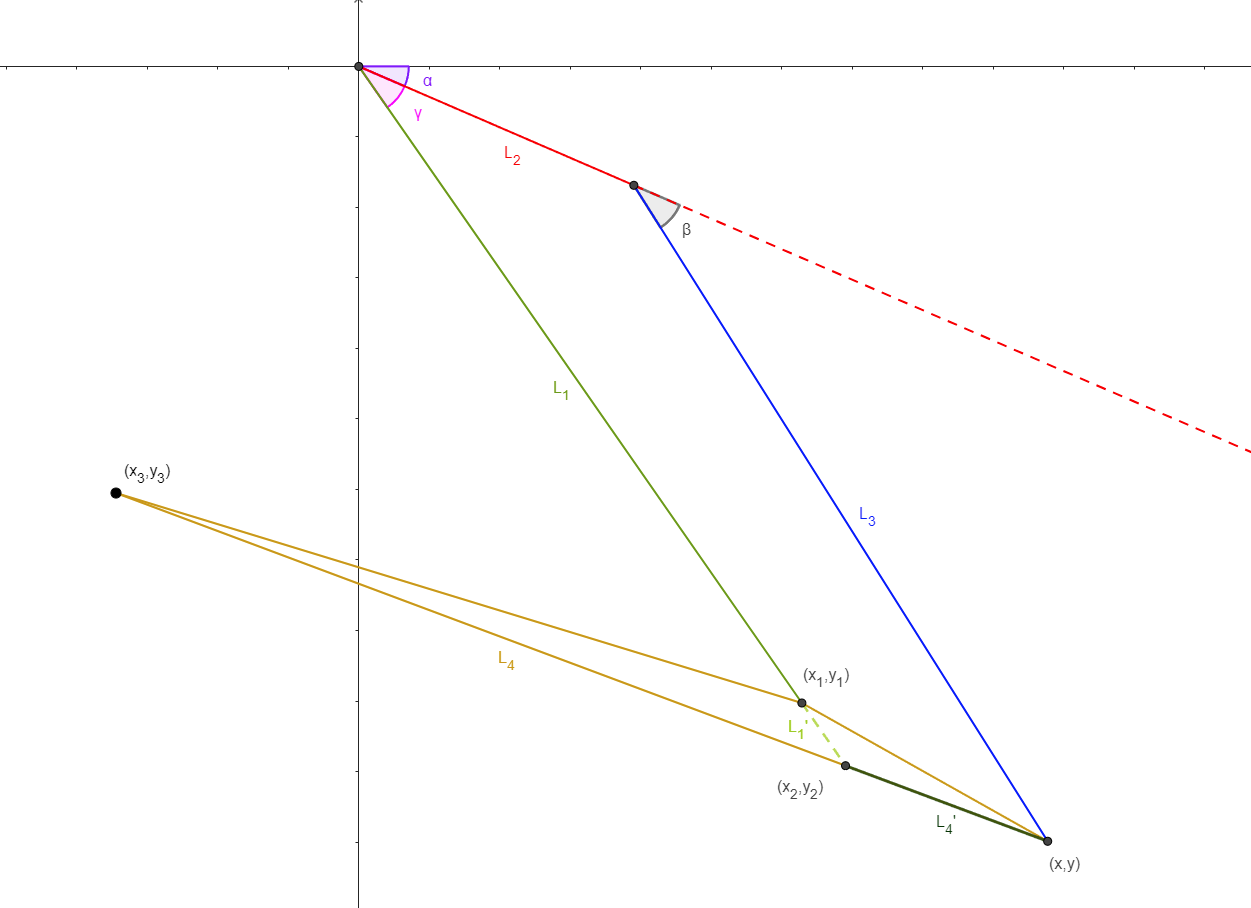
\includegraphics[angle=90,width=10cm]{Forward kinematics formula}
\caption{\Large 四連趕機構}\label{Forward kinematics formula}
\end{center}
\end{figure}

A部分:Leg1-1 + Leg1_5
B部分:Leg2 + Leg3
C部分:leg4

 %------------軟體架構-----------------%
\section{軟體架構}
運動模擬主要以Python程式碼進行控制,而程式碼部分我們選擇利用鍵盤控制模型的動作,首先將API模塊、keyboard模塊、time模塊導入(API模塊:遠端通訊、keyboard模塊:檢測鍵盤輸入、time模塊:暫停當前程式一段時間),接著將要控制的主機位置輸入,最後創建一個從遠端客戶端獲取的對象的變量,接下來就可以進行運動模擬控制,在仿生模擬中利用角度控制轉軸的所在位置,首先調用需要控制的轉軸,接著定義控制每隻轉軸的函數,再來設置一個無限迴圈檢測鍵盤是否按下設定的按鍵,最後將先前定義的函數寫入迴圈,將以上步驟完成後,即可控制每隻轉軸角度達成理想動作。設定前進動作:先將左前腿及右後腿往前抬,並同時將右前腿及左後腿往後踢,設定前抬左前腿時,左前腿的前抬角度必須比右後腿高,這樣才不會使左前腿觸碰到地面而造成反力無法前進,完成前面的動作後,將左右動作對調即可達成左右腿互換的動作。設定後退動作:先將左前腿及右後腿往後抬,並同時將右前腿及左後腿往前踢,設定後抬右後腿時,右後腿的後抬角度必須比左前腿高,這樣才不會使右後腿觸碰到地面而造成反力無法後退,完成前面的動作後,將左右動作對調即可達成左右腿互換的動作。\\
\newpage

%-----------運動學模擬------------%
\section{運動學模擬}
首先將模型轉化成STL檔案使其能被CoppeliaSim開啟,利用移動功能將模型移動至合適位置,點選模型使用爆炸功能將模型由一體分為數個零件,插入轉軸並設定中修改零件的重量等參數,導入Pythan程式碼,使用播放查看個機件的姿態、作動是否符合設計,完成之後就可以對模型進行分析並帶入負載求解。\\

\begin{figure}[hbt!]
\begin{center}
\includegraphics[scale=0.74]{clientProxy}
\caption{\Large clientProxy}\label{clientProxy}
\end{center}
\end{figure}

動態模擬結束後,我們可以將四足機器人運動模式分為以下三種,分別為:\

1. 爬行:\
此動作較簡單且容易控制,作用在於機器人需緩慢移動或是穩定度需求高的情況下,由其中單腳前伸其餘進行關節旋轉,在小位移量的情況下實現行走功能。\\

2. 小跑:\
此作用型態為FR+RL或FL+RR做動,進行移動時有著兩動兩不動的準則,在不動的部分做關節的旋轉運動,令四足機器人在快速移動下還能對身體保持平衡,在大位移量的情況下實現行走功能。\\

3. 跳躍:\
由前兩足進行快速彈跳位移,使機器狗的關節進行快速調整以支撐身體姿態,分為FL+FR及RL+RR兩組,在躍障或其他特殊行為中使用。\\

\begin{figure}[hbt!]
\begin{center}
\includegraphics[scale=0.74]{clientProxy}
\caption{\Large clientProxy}\label{clientProxy}
\end{center}
\end{figure}
\newpage

\chapter{四足機器人有限元素分析}

此專題以有限元素法作為主題,四足機器人為載體,目的就是為了使用有限元素法計算載體的受力後狀態,並利用了CoppeliaSim對模型進行了動態模擬,找出了各部件的最大力方向及位置。\
我們將單一步行機構負重定為六倍自身重量,為承受力630N,材質則選用了常見的PVE材料。\
分析環境選擇Solid Edge及Ansys同時進行,以利於對比資料並查看兩軟體區別。\\

\section{有限元素分析}
 下列圖示為個部位在Solid Edge中通過有限元素分析的步驟介紹:\\
 
1.開啟設計模型並切換到分析功能新增研究內容。\\

2.材料選擇3D列印機常用的PLA材質,在未來有需求時能夠及時並快速地做實體測驗並打印出模型。\\

3.依照原先設計者的參數設定負載為630N,為自身6倍體重。\\

4.通過CoppeliaSim找出個部位所受反力點及最大角度。\\

5.通過有限元素法出個部位受力狀態。\\

6.觀察求解後參數是否符合要求或是需要修改。\\

以上步驟為有限元素法通過電腦計算在四足機器狗上的應用,在每個設計者的作品誕生之初經常會使用到的分析,對於尋找產品缺陷或改進都有很大的幫助。\\
\newpage

\chapter{應力分析}
本專題已建立2D環境的算法與訓練數據,並將實體系統導入虛擬環境,建立跨平台控制(RemoteAPI)及輔助對打系統,後續可透過建立虛擬環境的訓練程式進行虛擬訓練,完成虛擬訓練後可導入實體機電系統,將對打系統實體化,架設伺服器提供網際介面,提供網際控制、即時觀看對打影像等功能。
\begin{figure}[hbt!]
\begin{center}
\includegraphics[width=16cm]{現有研究流程與未來展望}
\caption{\Large 現有研究流程與未來展望}
\label{fig.現有研究流程與未來展望}
\end{center}
\end{figure}

\chapter{總結}
\hspace{-1.7em} Q:gym用到的atari動態連結庫在讀取目錄下但在執行的時候出現缺少 ale\_ c.cp38-win\_ amd64.dll\\
\begin{figure}[hbt!]
\begin{center}
\includegraphics[width=15cm]{Q_dll}
\caption{\Large 動態連結庫錯誤}
\label{fig.動態連結庫錯誤}
\end{center}
\end{figure}
\newpage
\hspace{-1.4em}A:此問題尚未找到解決方法。\\
Q:錄製訓練過程的程式讀不到ffmpeg(圖.\ref{fig.Q_ffmpeg})。\\
\begin{figure}[hbt!]
\begin{center}
\includegraphics[width=15cm]{Q_ffmpeg}
\caption{\Large 程式讀不到ffmpeg}
\label{fig.Q_ffmpeg}
\end{center}
\end{figure}
\qquad \\
A:需要在作業系統中安裝ffmpeg:
\begin{enumerate}
\item 下載、解壓縮\\
先到官網 \href{https://ffmpeg.org/download.html}{https://ffmpeg.org/download.html} 下載" \href{https://www.gyan.dev/ffmpeg/builds/}{Windows builds from gyan.dev} ",下載 \href{https://www.gyan.dev/ffmpeg/builds/ffmpeg-git-full.7z}{https://www.gyan.dev/ffmpeg/builds/ffmpeg-git-full.7z} ,解壓縮重新命名成"ffmpeg"並放到C槽目錄下(C:$\setminus$ffmpeg)。
\item 環境設定(windows10 20H2 及 2004版本)\\
開啟"設定"→"系統"→左方"關於"選項→右側"進階系統設定"→"環境變數"(圖.\ref{fig.Q_ffmpeg-2})→選取"Path",編輯(圖.\ref{fig.Q_ffmpeg-3})→"新增",增加一個環境變數,給定內容為:"C:$\setminus$ffmpeg$\setminus$bin","確定"(圖.\ref{fig.Q_ffmpeg-4})→"確定"→"確定\\
\end{enumerate}
\begin{figure}[hbt!]
\begin{center}
\includegraphics[width=10cm]{Q_ffmpeg-2}
\caption{\Large 進階系統設定}
\label{fig.Q_ffmpeg-2}
\end{center}
\end{figure}
\fontsize{0.001pt}{1pt}\selectfont .\\ %圖片間距勿刪
\begin{figure}[hbt!]
\begin{center}
\includegraphics[width=10cm]{Q_ffmpeg-3}
\caption{\Large 環境變數}
\label{fig.Q_ffmpeg-3}
\end{center}
\end{figure}
\fontsize{0.001pt}{1pt}\selectfont .\\ %圖片間距勿刪
\newpage
\begin{figure}[hbt!]
\begin{center}
\includegraphics[width=15cm]{Q_ffmpeg-4}
\caption{\Large 編輯環境變數}
\label{fig.Q_ffmpeg-4}
\end{center}
\end{figure}
\fontsize{0.001pt}{1pt}\selectfont .\\ %圖片間距勿刪

\newpage %圖片間距勿刪
\fontsize{14pt}{28pt}\selectfont

\begin{itemize}
\item 測試\\
開啟命令字元(win+R,輸入"cmd"),執行"ffmpeg"(圖.\ref{fig.Q_ffmpeg-5})\\

\begin{figure}[hbt!]
\begin{center}
\includegraphics[width=15cm]{Q_ffmpeg-5}
\caption{\Large ffmpeg成功執行}
\label{fig.Q_ffmpeg-5}
\end{center}
\end{figure}
\end{itemize}
\newpage%圖片間距勿刪
\hspace{-1.7em} Q:運用gym.wrappers.Monitor透過ffmpeg進行錄影,紀錄下訓練影像。但記錄後的影像資料皆為1KB,並且無法開啟。(圖.\ref{fig.ffmpeg_mp4})\\
\begin{figure}[hbt!]
\begin{center}
\includegraphics[width=15cm]{ffmpeg_mp4}
\caption{\Large 錄製後,影片無法開啟}
\label{fig.ffmpeg_mp4}
\end{center}
\end{figure}
\qquad \\%圖片間距勿刪
%圖片間距勿刪
A:修改g ym.wrappers.Monitor的video\_ recorder.py的設定(圖.\ref{fig.video_recorder}),將303行的縮排修正(從if階層上移到def的階層)即可(圖.)。\\
\begin{figure}[hbt!]
\begin{center}
\includegraphics[width=15cm]{video_recorder}
\caption{\Large 原始設定}
\label{fig.video_recorder}
\end{center}
\end{figure}

\begin{figure}[hbt!]
\begin{center}
\includegraphics[width=15cm]{修正video_recorder}
\caption{\Large 修正後設定}
\label{fig.修正video_recorder}
\end{center}
\end{figure}
\newpage %圖片間距勿刪

\hspace{-1.7em} Q:啟用cmsimde的MathJax的功能遇到文章使用括號補充說明的內容被誤當成latex的語法轉換。\\
\hspace{-1.7em} A:格式轉換原始定義成"("和")",所以出現誤換的問題。\\
\begin{lstlisting}[caption=\Large\sectionef MathJax 程式碼]
<script>
  MathJax = {
    tex: {inlineMath: [['$', '$'], ['\\(', '\\)']]}
  };
  </script>
  <script id="MathJax-script" 
  async src="https://cdn.jsdelivr.net/npm/mathjax@3/es5/tex-chtml.js"> 
  </script>
\end{lstlisting}

修正後將"("和")"換成"\$",就解決誤換問題

%=---------------------參考文獻----------------------=%
\input{9_reference.tex}
%=---------------附錄-----------------=%
\addcontentsline{toc}{chapter}{附錄} %新增目錄名稱
\begin{appendix}
\renewcommand{\thesection}{\bf 附錄 \Alph{section}}%設定標題名稱
\begin{center}
\fontsize{20pt}{0em}\selectfont\bf 附錄
\end{center}
\section*{LaTeX}
LaTex 為一種程式語言,支援標準庫 (Standard Libraries) 和外部程式庫 (External Libraries),不過與一般程式語言不同的是,它可以直接表述 Tex 排版結構,類似於 PHP 之於 HTML 的概念。但是直接撰寫 LaTex 仍較複雜,因此可以藉由 Markdown 這種輕量的標註式語言先行完成文章,再交由 LaTex 排版。
此專題報告採用編輯軟體為LaTeX,綜合對比Word編輯方法,LaTeX較為精準正確、更改、製作公式等,以便符合規範、製作。
 \begin{table}[htbp] %htbp代表表格浮動位置
			\centering%表格居中
			\caption{文字編輯軟體比較表}%表:標題
			\large%字體大小
			\label{tab_文字編輯軟體比較表:scale}
			\begin{tabular}{|c|c|c|c|c|c|c|}
			\hline
			\diagbox[width=5em]& 相容性 & 直觀性 & 文件排版 & 數學公式 & 微調細部\\ 
			\hline
			LaTeX 		&$\surd$&		&$\surd$&$\surd$&$\surd$\\
			\hline
			Word	 	&		&$\surd$&		&		&$\surd$\\
			\hline
			
			\end{tabular}
		\end{table}	

\begin{itemize} 
\item 特點:
\end{itemize}
\begin{enumerate}
\item 相容性:以Word為例會有版本差異,使用較高版本編輯的文件可能無法以較低的版本開啟,且不同作業系統也有些許差異;相比LaTeX可以利用不同編譯器進行編譯,且為免費軟體也可移植至可攜系統內,可以搭配Github協同編譯。
\item 文件排版:許多規範都會要求使用特定版型,使用文字編譯環境較能準確符合規定之版型,且能夠大範圍的自定義排定所需格式,並能不受之後更改而整體格式變形。
\item 數學公式呈現:LaTex可以直接利用本身多元的模組套件加入、編輯數學公式,在數學推導過程能夠快速的輸入自己需要的內容即可。
\item 細部調整:在大型論文、報告中有多項文字、圖片、表格,需要調整細部時,要在好幾頁中找尋,而LaTeX可以分段章節進行編譯,再進行合併處理大章節。
\end{enumerate}

\section*{FFmpeg}
FFmpeg是一個開放原始碼的自由軟體,可以對音訊和視訊進行多種格式的錄影、轉檔、串流功能。在專題訓練過程中透過FFmpeg的視訊錄製的功能記錄對打影像來了解實際訓練狀況。
\newpage

\newpage
%=-------------作者簡介-----------------=%
    \addcontentsline{toc}{chapter}{作者簡介}
    \begin{center}
	\fontsize{20pt}{0em}\selectfont \bf{作者簡介}\\
	\end{center}	
	{\begin{textblock}{6}(0,0.5)
	\begin{figure}
	\includegraphics[width=1.25in]{40923231}
	\end{figure}
	\end{textblock}}
	{\renewcommand\baselinestretch{0.99}\selectfont %設定以下行距
	{\begin{textblock}{15}(3.5,0.7)%{寬度}(以左上角為原點之右移量,下移量)
	\noindent\fontsize{14pt}{0em}\selectfont \makebox[4em][s]{姓名}\enspace:\enspace
    \fontsize{14pt}{0em}\selectfont \makebox[4em][s]{楊子頡}\\     \hspace*{\fill} \\
    \fontsize{14pt}{0em}\selectfont \makebox[4em][s]{學號}\enspace:\enspace
    \fontsize{14pt}{0em}\selectfont \makebox[4em][s]{40923231} \\ %\makebox為文本盒子
    \hspace*{\fill} \\
    \fontsize{14pt}{0em}\selectfont \makebox[4em][s]{畢業學校}\enspace:\enspace
    \fontsize{14pt}{0em}\selectfont \makebox[9em][s]{國立虎尾科技大學}\\
    \fontsize{14pt}{0em}\selectfont \makebox[5em][s]{\quad}\enspace\enspace
    \fontsize{14pt}{0em}\selectfont \makebox[8em][s]{機械設計工程系}\\
    \hspace*{\fill} \\
    \fontsize{14pt}{0em}\selectfont \makebox[4em][s]{經歷}\enspace:\enspace
    \end{textblock}}}
   % \hspace*{\fill} \\
   \vspace{2em}
	{\begin{textblock}{6}(0,2.3)
	\begin{figure}
	\includegraphics[width=1.15in]{40923233} 
    \end{figure}
    \end{textblock}}
    {\renewcommand\baselinestretch{0.99}
    \selectfont %設定以下行距
    {\begin{textblock}{15}(3.5,2.5) %{寬度}(以左上角為原點之右移量,下移量)
\noindent\fontsize{14pt}{0em}\selectfont \makebox[4em][s]{姓名}\enspace:\enspace
\fontsize{14pt}{0em}\selectfont \makebox[4em][s]{楊建霖}\\ 
\hspace*{\fill} \\
\fontsize{14pt}{0em}\selectfont \makebox[4em][s]{學號}\enspace:\enspace
\noindent\fontsize{14pt}{0em}\selectfont \makebox[4em][s]{40923233} \\ 
\hspace*{\fill} \\
\fontsize{14pt}{0em}\selectfont \makebox[4em][s]{畢業學校}\enspace:\enspace
\fontsize{14pt}{0em}\selectfont \makebox[9em][s]{國立虎尾科技大學}\\
\fontsize{14pt}{0em}\selectfont \makebox[5em][s]{\quad}\enspace\enspace
\fontsize{14pt}{0em}\selectfont \makebox[8em][s]{機械設計工程系}\\
\hspace*{\fill} \\
\fontsize{14pt}{0em}\selectfont \makebox[4em][s]{經歷}\enspace:\enspace
    \end{textblock}}}
    %\hspace*{\fill} \\
    \vspace{2em}
    {\begin{textblock}{6}(0,4.1)
    \begin{figure}
        \includegraphics[width=1.15in]{40923235} %{}內是圖片文件的相對路徑
    \end{figure}
    \end{textblock}}
    {\renewcommand\baselinestretch{0.99}\selectfont %設定以下行距
    {\begin{textblock}{15}(3.5,4.3) %{寬度}(以左上角為原點之右移量,下移量)
\noindent\fontsize{14pt}{0em}\selectfont \makebox[4em][s]{姓名}\enspace:\enspace%\noindent指定首行不進行縮排
\fontsize{14pt}{0em}\selectfont \makebox[4em][s]{詹侑儒}\\ 
\hspace*{\fill} \\
\noindent\fontsize{14pt}{0em}\selectfont \makebox[4em][s]{學號}\enspace:\enspace
\noindent\fontsize{14pt}{0em}\selectfont \makebox[4em][s]{40923235} \\ %\makebox為文本盒子
\hspace*{\fill} \\
\noindent\fontsize{14pt}{0em}\selectfont \makebox[4em][s]{畢業學校}\enspace:\enspace
\noindent\fontsize{14pt}{0em}\selectfont \makebox[9em][s]{國立虎尾科技大學}\\
\noindent\fontsize{14pt}{0em}\selectfont \makebox[5em][s]{\quad}\enspace\enspace
\noindent\fontsize{14pt}{0em}\selectfont \makebox[8em][s]{機械設計工程系}\\
\hspace*{\fill} \\
\noindent\fontsize{14pt}{0em}\selectfont \makebox[4em][s]{經歷}\enspace:\enspace
    \end{textblock}}}
   % \hspace*{\fill} \\
   \vspace{2em}
    {\begin{textblock}{6}(0,5.9)
    \begin{figure}
        \includegraphics[width=1.15in]{} %{}內是圖片文件的相對路徑
    \end{figure}
    \end{textblock}}
    {\renewcommand\baselinestretch{0.99}\selectfont %設定以下行距
    {\begin{textblock}{15}(3.5,6.1) %{寬度}(以左上角為原點之右移量,下移量)
\noindent\noindent\fontsize{14pt}{0em}\selectfont \makebox[4em][s]{姓名}\enspace:\enspace
\noindent\fontsize{14pt}{0em}\selectfont \makebox[4em][s]{蔡宗瑋}\\ \hspace*{\fill} \\
\noindent\fontsize{14pt}{0em}\selectfont \makebox[4em][s]{學號}\enspace:\enspace
\noindent\fontsize{14pt}{0em}\selectfont \makebox[4em][s]{40923240} \\ \hspace*{\fill} \\
\noindent\fontsize{14pt}{0em}\selectfont \makebox[4em][s]{畢業學校}\enspace:\enspace
\noindent\fontsize{14pt}{0em}\selectfont \makebox[9em][s]{國立虎尾科技大學}\\
\noindent\fontsize{14pt}{0em}\selectfont \makebox[5em][s]{\quad}\enspace\enspace
\noindent\fontsize{14pt}{0em}\selectfont \makebox[8em][s]{機械設計工程系}\\
\hspace*{\fill} \\
\noindent\fontsize{14pt}{0em}\selectfont \makebox[4em][s]{經歷}\enspace:\enspace
    \end{textblock}}}
\newpage
%=----------------書背----------------------=%
\pagestyle{empty}%設定沒有頁眉和頁腳
\begin{center}
\fontsize{0.001pt}{1pt}\selectfont .\\
\vspace{4em}
\fontsize{30pt}{30pt}\selectfont 【13】 \\
\fontsize{20pt}{20pt}\selectfont
\vspace{0.5em}
分\\
類\\
編\\
號\\
\vspace{0.5em}
\hspace{-0.5em}:\\
\vspace{0.5em}
\rotatebox[origin=cc]{270}{\sectionef\LARGE \textbf{109-4-APP-3004-1}}\\ %旋轉
\vspace{0.5em}
有\\
限\\
元\\
素\\
法\\
在\\
四\\
足\\
機\\
器\\
人\\
上\\
的\\
應\\
用\\
\vspace{2em}
一\\
一\\
貳\\
級\\

\end{center}
%\newpage
%\begin{landscape}  %橫式環境
%\begin{center}
%\fontsize{0.001pt}{1pt}\selectfont .
%\vspace{70mm}
%\rotatebox[origin=cc]{90}{\LARGE 【14】}\rotatebox[origin=cc]%{180}{\LARGE 1-2-APP-8765} %旋轉
%\end{center}
%\end{landscape}
\end{document}
